\documentclass[a4paper, parskip=half]{scrartcl}

\usepackage[sfdefault,light]{roboto}
\usepackage{inconsolata}
\usepackage[english]{babel}

\usepackage[utf8]{inputenc}
\usepackage[T1]{fontenc}

\usepackage{currfile}

\usepackage{microtype}

\usepackage{csquotes}
\MakeOuterQuote{"}

\usepackage{listings}

\usepackage{graphicx}
\usepackage{float}
\usepackage{bm}
\graphicspath{./entwurf/}

\usepackage{tikz}
\usetikzlibrary{arrows, arrows.meta}

\usepackage[hidelinks]{hyperref}

\lstset{basicstyle=\ttfamily}

\newcommand{\lnk}[1]{\hyperref[type:\pkg.#1]{#1}}
\newcommand{\pkg}{\currfilebase}
\newcommand{\pkglnk}[1]{\hyperref[pkg:edu.kit.wavelength.client.#1]{#1}}

%\title{THE DESIGN}

\titlehead{\centering
\includegraphics[width=6cm]{img/logo.pdf}}
\title{Design Document}
\subtitle{Wavelength --- $\bm{\lambda}$-IDE}
\author{Muhammet Guemues, Markus Himmel, Marc Huisinga,\\Philip Klemens, Julia Schmid, Jean-Pierre von der Heydt}


\begin{document}
\maketitle
\thispagestyle{empty}
\newpage
\tableofcontents
\newpage
\section{Introduction}

This document contains the design for "Wavelength", a web-based IDE for the untyped
lambda calculus, as described in the \textit{Pflichtenheft}.

The object-oriented architecture of the project roughly follows the model-view-controller (MVC)
architectural pattern. It consists of two largely independent sets of packages: \texttt{model} and \texttt{view}.
The architecture differs from MVC in the sense that there is no communication between views and models, 
all communication between the two passes through the respective controller. 
Additionally the controller is divided into two parts: \texttt{action} and \texttt{update}. 
\texttt{action} handles user inputs from the view, while \texttt{update} handles concurrent updates from other sources, for instance the model.
At the center of the architecture is the \texttt{\hyperref[type:edu.kit.wavelength.client.view.App]{App}} class, which initializes and holds the view. 
\texttt{action} and \texttt{update} both query \texttt{\hyperref[type:edu.kit.wavelength.client.view.App]{App}} for the view elements it holds.
As a result of this architecture, the entirety of the model is decoupled from the view and the rest of the application.

\begin{figure}[h]
	\centering
	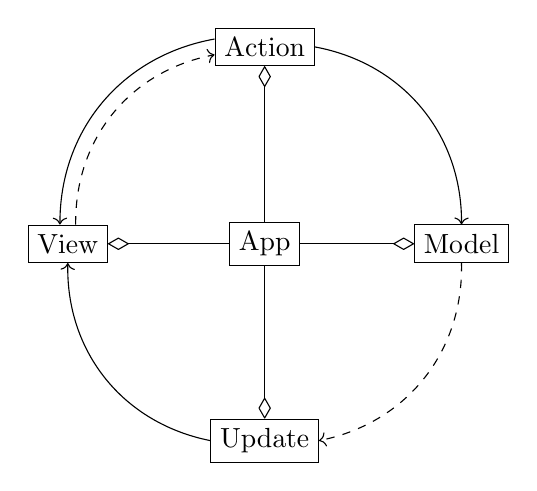
\begin{tikzpicture}
		\node[rectangle, draw] (app) at (0, 0) {App};
		\node[rectangle, draw] (model) at (2.5, 0) {Model};
		\node[rectangle, draw] (view) at (-2.5, 0) {View};
		\node[rectangle, draw] (action) at (0, 2.5) {Action};
		\node[rectangle, draw] (update) at (0, -2.5) {Update};

		\draw[-{open diamond}] (app) -- (view);
		\draw[-{open diamond}] (app) -- (model);
		\draw[-{open diamond}] (app) -- (action);
		\draw[-{open diamond}] (app) -- (update);

		\draw[->] (action.east) to[bend left=40] (model.north);
		\draw[->,dashed] (model.south) to[bend left=40] (update.east);
		\draw[->] (update.west) to[bend left=40] (view.south);
		\draw[->,dashed] ([xshift=0.1cm]view.north) to[bend left=40] ([yshift=-0.1cm]action.west);
		\draw[->] ([yshift=0.1cm]action.west) to[bend right=40] ([xshift=-0.1cm]view.north);
	\end{tikzpicture}
	\caption{Sketch of the application architecture. Actions are indirectly called by the view
	and updates are indirectly called by the model. Actions interact with the view and control the model,
	while updates update the view. \texttt{\hyperref[type:edu.kit.wavelength.client.view.App]{App}} initializes 
	the application and provides access to the view to
		actions and updates.}
\end{figure}

\subsection{The model}

The first set of packages (\texttt{\pkglnk{model}} and its subpackages) comprises most of the model 
and provides means for interactively, but
synchronously, operating on lambda terms. It is designed as a library that makes few
assumptions about how it is used.

It provides a package with a very general set of classes representing
\texttt{\hyperref[type:edu.kit.wavelength.client.model.term.LambdaTerm]{LambdaTerm}}s as a 
tree structure of immutable objects. For operations on these
lambda terms, the visitor pattern is utilized. Since many operations performed on 
lambda terms fall into a few categories (for example displaying terms in some way or transforming a 
term into another term), some special abstract visitors are provided in order to make these common
operations less cumbersome. For the most fundamental operations on 
lambda terms, concrete visitors are provided, but the 
\texttt{\hyperref[type:edu.kit.wavelength.client.model.term.Visitor]{Visitor}} interface may be 
implemented by any entity wishing to operate on lambda terms (for instance reduction orders or the 
user interface for displaying
terms).

In addition to \texttt{\hyperref[type:edu.kit.wavelength.client.model.term.LambdaTerm]{LambdaTerm}}s 
and visitors and the ability to parse strings into
\texttt{\hyperref[type:edu.kit.wavelength.client.model.term.LambdaTerm]{LambdaTerm}}s, the model 
provides interfaces for reduction orders,
output sizes and libraries as well as the implementations of the concrete reductions orders,
output sizes and libraries mentioned in the \textit{Pflichtenheft}. These three
concepts are each fully contained in separate packages which only use the package
providing \texttt{\hyperref[type:edu.kit.wavelength.client.model.term.LambdaTerm]{LambdaTerm}}s.

%TODO besseres englisch
The central interface of the model to the user interface is the 
\texttt{\hyperref[type:edu.kit.wavelength.client.view.execution.Executor]{Executor}} wrapping the
\texttt{\hyperref[type:edu.kit.wavelength.client.model.ExecutionEngine]{ExecutionEngine}}
class, which manages the state of an interactive reduction of a lambda term. It
keeps the current state and history of the execution and allows performing the next
reduction step, either of a supplied redex or according to the currently set reduction
order.

\subsection{The user interface}

The second set of packages (\texttt{\pkglnk{view}} and its subpackages) manages building the user 
interface (UI) and enabling UI elements to interact with the model.

In order to abstract the necessary aspects of UI elements the \texttt{\pkglnk{view.api}} package 
defines elementary interfaces.
For a further narrowing of aspects the \texttt{\pkglnk{view.webui.component}} package wraps some of 
GWT's widgets using the adapter pattern.

Regarding user interaction the UI elements are able to run actions as specified in the 
\texttt{\hyperref[type:edu.kit.wavelength.client.view.action.Action]{Action}} interface when used (on click for example).
Actions are supposed to cover an abundance of manipulations on other UI elements or even the model.

Since providing concurrency for the reduction of lambda terms is crucial for maintaining responsiveness of the UI 
the \texttt{\pkglnk{view.execution}} package provides a wrapper class for the \texttt{\hyperref[type:edu.kit.wavelength.client.model.ExecutionEngine]{ExecutionEngine}} class and an associated
observer interface.

The communication between the view and the model is handled by the \texttt{\hyperref[type:edu.kit.wavelength.client.view.App]{App}} class. It stores all available UI elements and
an \texttt{\hyperref[type:edu.kit.wavelength.client.view.execution.Executor]{Executor}} (wrapping an \texttt{\hyperref[type:edu.kit.wavelength.client.model.ExecutionEngine]{ExecutionEngine}}) and provides access to them. 
This feature is essential for actions giving them easy access to resources.
The general \texttt{\pkglnk{view}} package provides the \texttt{\hyperref[type:edu.kit.wavelength.client.view.App]{App}} class but also a 
\texttt{\hyperref[type:edu.kit.wavelength.client.view.URLSerializer]{URLSerializer}} class for serializing a URL and the associated Observer class.

The \texttt{\pkglnk{view.update}} package provides concrete observers for serialization and execution along with
visitors for resolving lambda terms according to different outputFormats.

The \texttt{\pkglnk{view.export}} package provides means of transforming the output to a specific Format.

Lastly there is an exercise mode available represented by the \texttt{\pkglnk{view.exercise}} package providing
an interface, a concrete implementation and a static list of all exercises.

\pagebreak
\section{Packages and classes}
\documentclass[11pt,a4paper]{article}
\usepackage{color}
\usepackage{ifthen}
\usepackage{ifpdf}
\usepackage[headings]{fullpage}
\usepackage{listings}
\lstset{language=Java,breaklines=true}
\ifpdf \usepackage[pdftex, pdfpagemode={UseOutlines},bookmarks,colorlinks,linkcolor={blue},plainpages=false,pdfpagelabels,citecolor={red},breaklinks=true]{hyperref}
  \usepackage[pdftex]{graphicx}
  \pdfcompresslevel=9
  \DeclareGraphicsRule{*}{mps}{*}{}
\else
  \usepackage[dvips]{graphicx}
\fi

\newcommand{\entityintro}[3]{%
  \hbox to \hsize{%
    \vbox{%
      \hbox to .2in{}%
    }%
    {\bf  #1}%
    \dotfill\pageref{#2}%
  }
  \makebox[\hsize]{%
    \parbox{.4in}{}%
    \parbox[l]{5in}{%
      \vspace{1mm}%
      #3%
      \vspace{1mm}%
    }%
  }%
}
\newcommand{\refdefined}[1]{
\expandafter\ifx\csname r@#1\endcsname\relax
\relax\else
{$($in \ref{#1}, page \pageref{#1}$)$}\fi}
\date{\today}
\chardef\textbackslash=`\\
\title{Der Entwurf}

\usepackage[sfdefault,light]{roboto}
\usepackage{inconsolata}

\lstset{basicstyle=\ttfamily}

\begin{document}
\sloppy
\addtocontents{toc}{\protect\markboth{Contents}{Contents}}
\tableofcontents
\section{Package edu.kit.wavelength.model.terms}{
\label{edu.kit.wavelength.model.terms}\hypertarget{edu.kit.wavelength.model.terms}{}
\hskip -.05in
\hbox to \hsize{\textit{ Package Contents\hfil Page}}
\vskip .13in
\hbox{{\bf  Classes}}
\entityintro{LambdaTerm}{edu.kit.wavelength.model.terms.LambdaTerm}{Represents a term in the untyped lambda calculus.}
\vskip .1in
\vskip .1in
\subsection{\label{edu.kit.wavelength.model.terms.LambdaTerm}Class LambdaTerm}{
\hypertarget{edu.kit.wavelength.model.terms.LambdaTerm}{}\vskip .1in 
Represents a term in the untyped lambda calculus.\vskip .1in 
\subsubsection{Declaration}{
\begin{lstlisting}[frame=none]
public class LambdaTerm
 extends java.lang.Object\end{lstlisting}
\subsubsection{Constructor summary}{
\begin{verse}
\hyperlink{edu.kit.wavelength.model.terms.LambdaTerm()}{{\bf LambdaTerm()}} \\
\end{verse}
}
\subsubsection{Constructors}{
\vskip -2em
\begin{itemize}
\item{ 
\index{LambdaTerm()}
\hypertarget{edu.kit.wavelength.model.terms.LambdaTerm()}{{\bf  LambdaTerm}\\}
\begin{lstlisting}[frame=none]
public LambdaTerm()\end{lstlisting} %end signature
}%end item
\end{itemize}
}
}
}
\end{document}


\section{Amendments to the requirements laid out in the \textit{Pflichtenheft}}

Regarding entry F17 in the "Pflichtenheft":
Enabling test cases raises complexity too much to be considered at this point of time.
According to F17 it is possible that an exercises gives predefined variables which
are set in the test cases. This leads to the problem that in order for a substitution of
those variables some kind of pre-parser needs to be utilized.
Hence the decision to not implement test cases for Exercises.

\section{Typical processes}
\subsection{Initialization of application}
%---------------------------
%include sequence diagram for initialization here
%---------------------------

\subsection{example action: select export format}
This sequence diagram states as example for a simple action handler.
In this action the user wants the currently displayed output translated into a specified format. The sequence diagram starts when the user selects the export format in the UI. 
The SelectExportFormat poses as action handler for the selected UI element. Thus when this element is clicked, the actions run() method is called. All invoked instances are already existing, none is being created in this scenario.
The actions run() method generates the dedicated representation by requesting the currently displayed lambda terms from the ExecutionEngine instance and generating their representation.
The representation is then written into the export window that will be displayed to the user. Writing before showing this export window ensures, that at no point in time an empty window is displayed.
However, before actually displaying it, a blocker that prevents the user from interacting with any UI element, other than the export window, is enabled.

\begin{figure}[H]
	\centering
	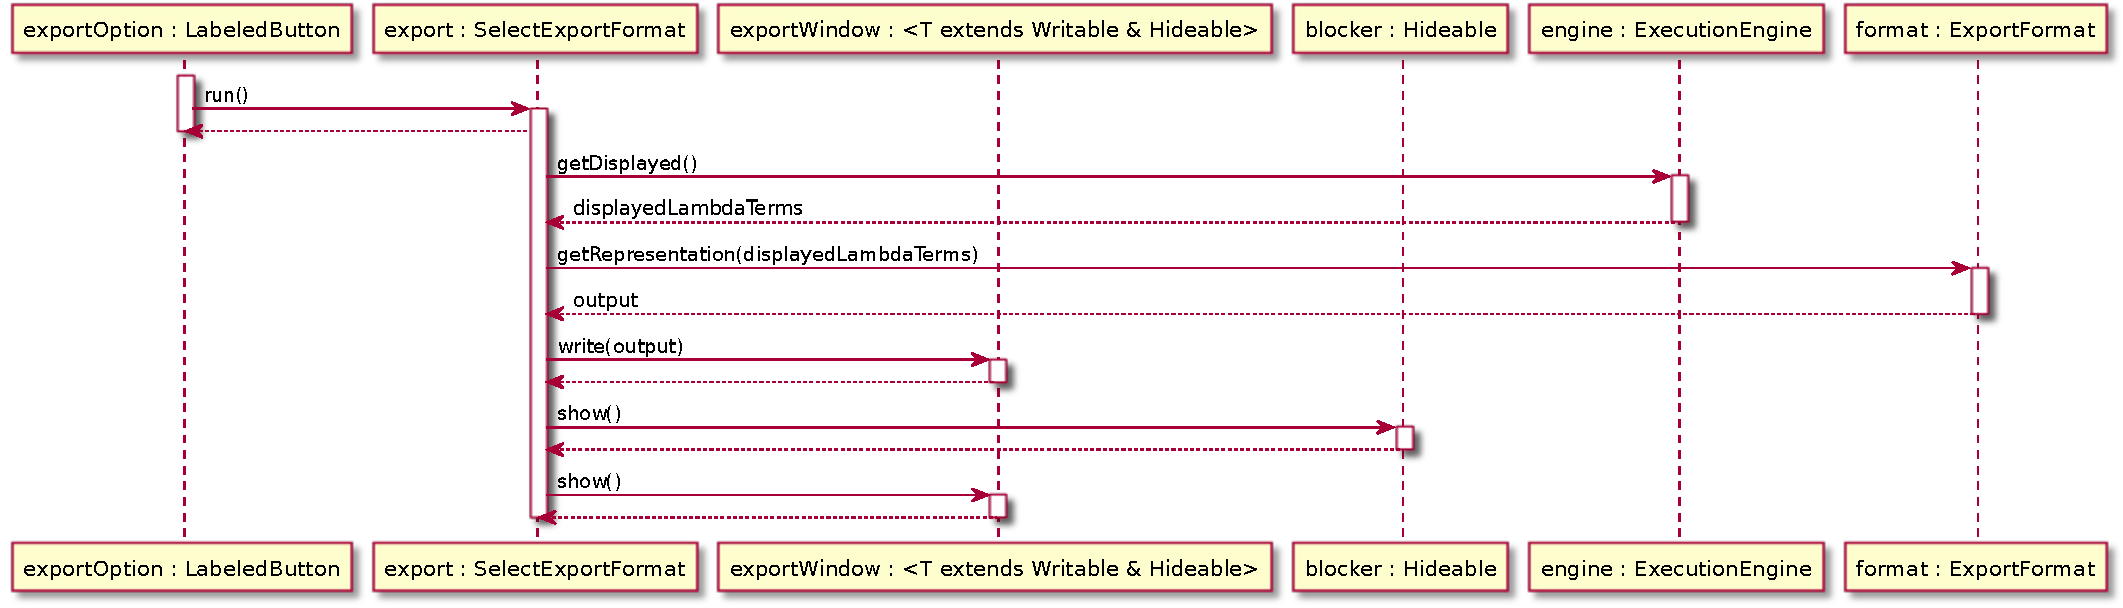
\includegraphics[width=\textwidth]{sequenceDiagrams/exportOutput}
	\caption{Sequence diagram for the select export format action.}
\end{figure}

\subsection{example action: select exercise from main menu}
The \texttt{\hyperref[type:edu.kit.wavelength.client.view.action.SelectExercise]{SelectExercise}} 
action handles the UI elements, when the user selects an exercise from the main menu.

This action only prepares the UI to display the content of the selected exercise, 
it does not load the actual content into the UI. If the content of the editor would 
be overridden when the selected exerciser is loaded, the action displays a warning
message. Otherwise it just calls the \texttt{\hyperref[type:edu.kit.wavelength.client.view.action.LoadExercise]{LoadExercise}} 
action which will in return load the selected exercise.

%\begin{figure}[H]
%	\centering
%	\includegraphics[width=\textwidth]{sequenceDiagrams/}
%	\caption{Sequenze diagram for selecting an exercise form the main menu.}
%\end{figure}

\subsection{example action: load selected exercise}
The \texttt{\hyperref[type:edu.kit.wavelength.client.view.action.LoadExercise]{LoadExercise}} 
action loads a selected Exercise into the UI.

It updates the width of the Editor and displays \texttt{\hyperref[type:edu.kit.wavelength.client.view.webui.component.TextField]{TextField}}s 
that are responsible for displaying solution and explanation of the exercise.
The action also writes the correct content into the \texttt{\hyperref[type:edu.kit.wavelength.client.view.webui.component.TextField]{TextField}}s and updates the content of the \texttt{\hyperref[type:edu.kit.wavelength.client.view.webui.component.Editor]{Editor}} if necessary.

%\begin{figure}[H]
%	\centering
%	\includegraphics[width=\textwidth]{sequenceDiagrams/}
%	\caption{Sequenze diagram for loading a selected exercise into the UI}
%\end{figure}

\subsection{Next term}
\label{sec:nt}
In order to retrieve the next redex to reduce from its reduction order, the
\texttt{\hyperref[type:edu.kit.wavelength.client.model.ExecutionEngine]{ExecutionEngine}}
calls the \texttt{next} method on the current reduction order. This method creates a new visitor which traverses
the lambda term, looking for the correct redex. In order to identify redexes,
specialized visitors that determine the type of a given lambda term are used.
These visitors extend \texttt{\hyperref[type:edu.kit.wavelength.client.model.term.NameAgnosticVisitor]{NameAgnosticVisitor}},
so that for example a named redex is still recognized as a redex.



\begin{figure}[H]
	\centering
	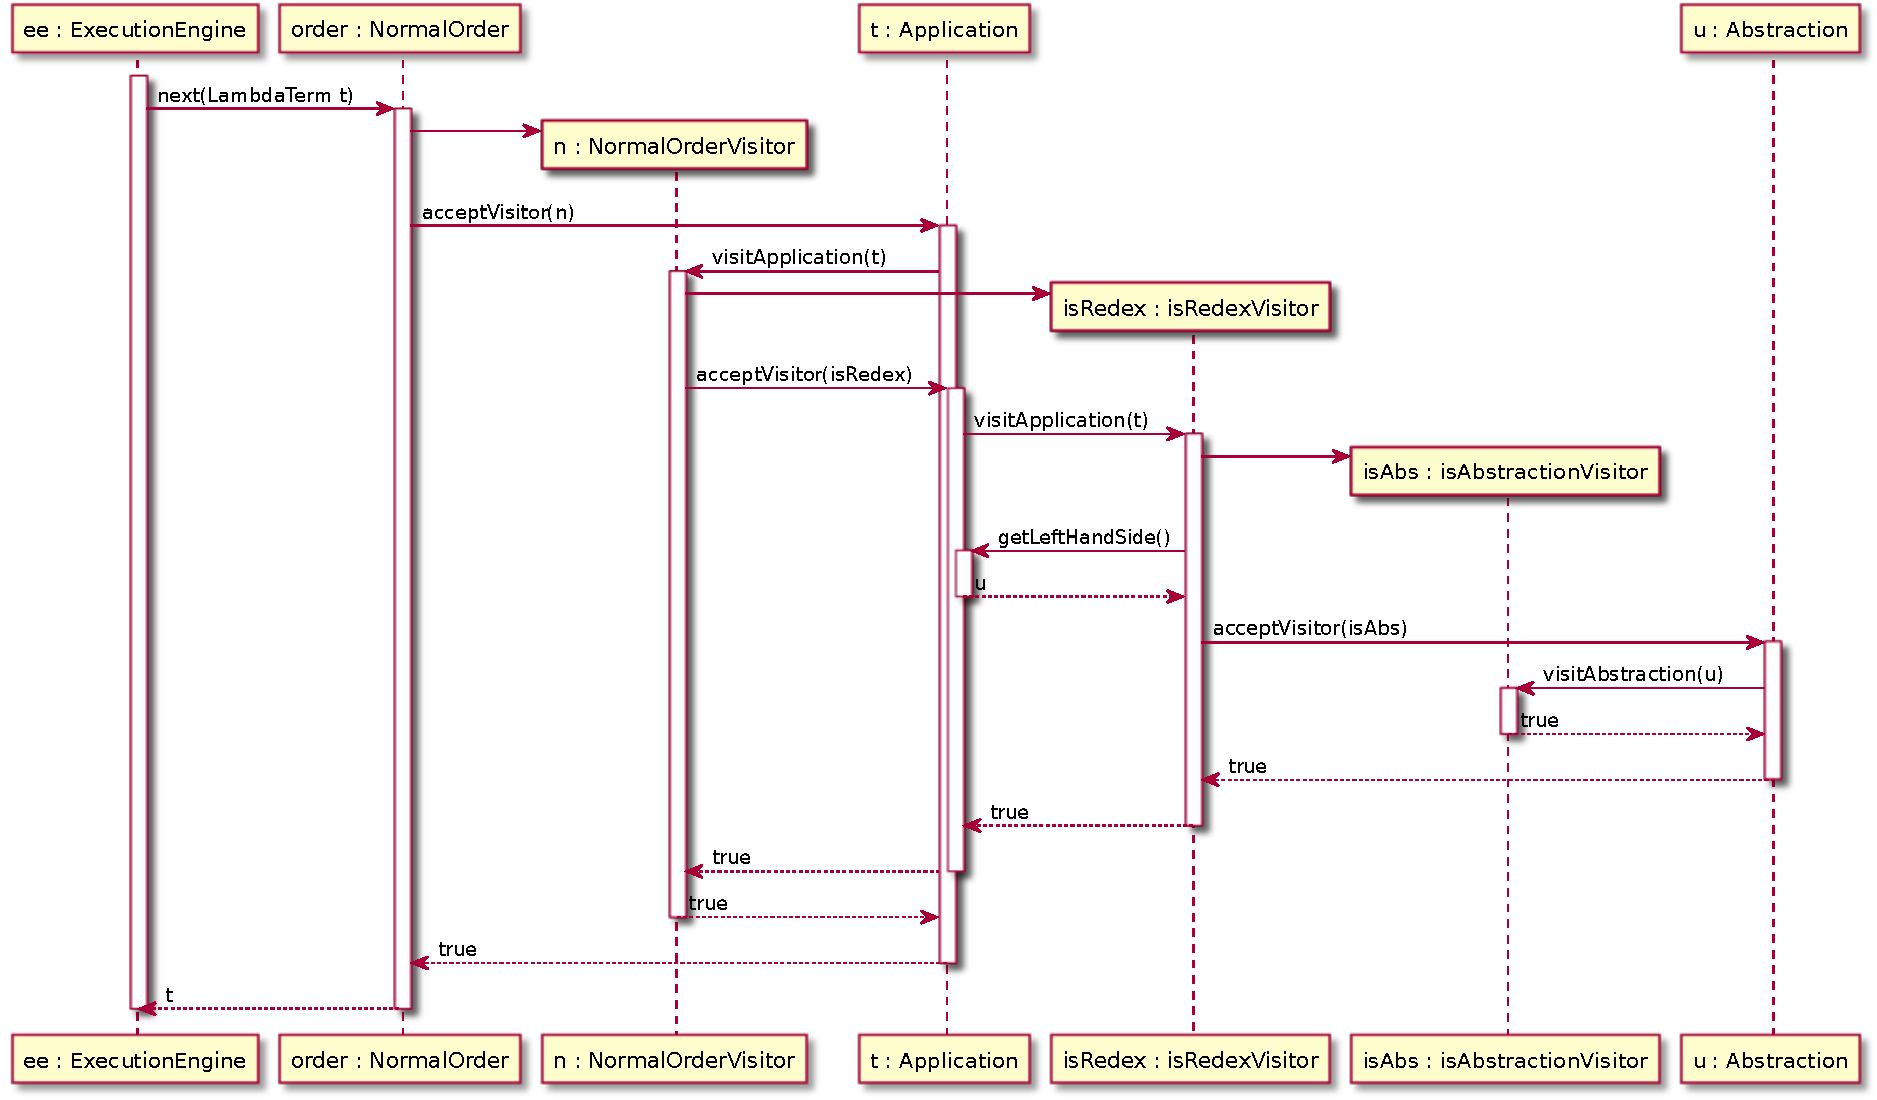
\includegraphics[width=\textwidth]{sequenceDiagrams/nextTerm}
	\caption{Sequence diagram for choosing the next term to reduce. In this example, we have $t = (\lambda x.x)(\lambda x.x)$ and $u = \lambda x.x$.}
\end{figure}


\subsection{$\beta$-reduction}
After the next redex to reduce has been retrieved from the reduction order (see \ref{sec:nt}),
the $\beta$-reduction of the redex can take place. Reduction is performed by the
\texttt{\hyperref[type:edu.kit.wavelength.client.model.term.BetaReducer]{BetaReducer}}
class, which traverses the tree and reassembles it unchanged until it finds the
redex returned by the reduction order. It then creates a
\texttt{\hyperref[type:edu.kit.wavelength.client.model.term.SubstitutionVisitor]{SubstitutionVisitor}}
which traverses the abstraction and performs the actual substitution. Both classes
extend \texttt{\hyperref[type:edu.kit.wavelength.client.model.term.TermTransformer]{TermTransformer}},
so they make sure that if they encounter a \texttt{\hyperref[type:edu.kit.wavelength.client.model.term.NamedTerm]{NamedTerm}}
whose body changed as a result of the substitution, the name tag is removed.


\begin{figure}[H]
	\centering
	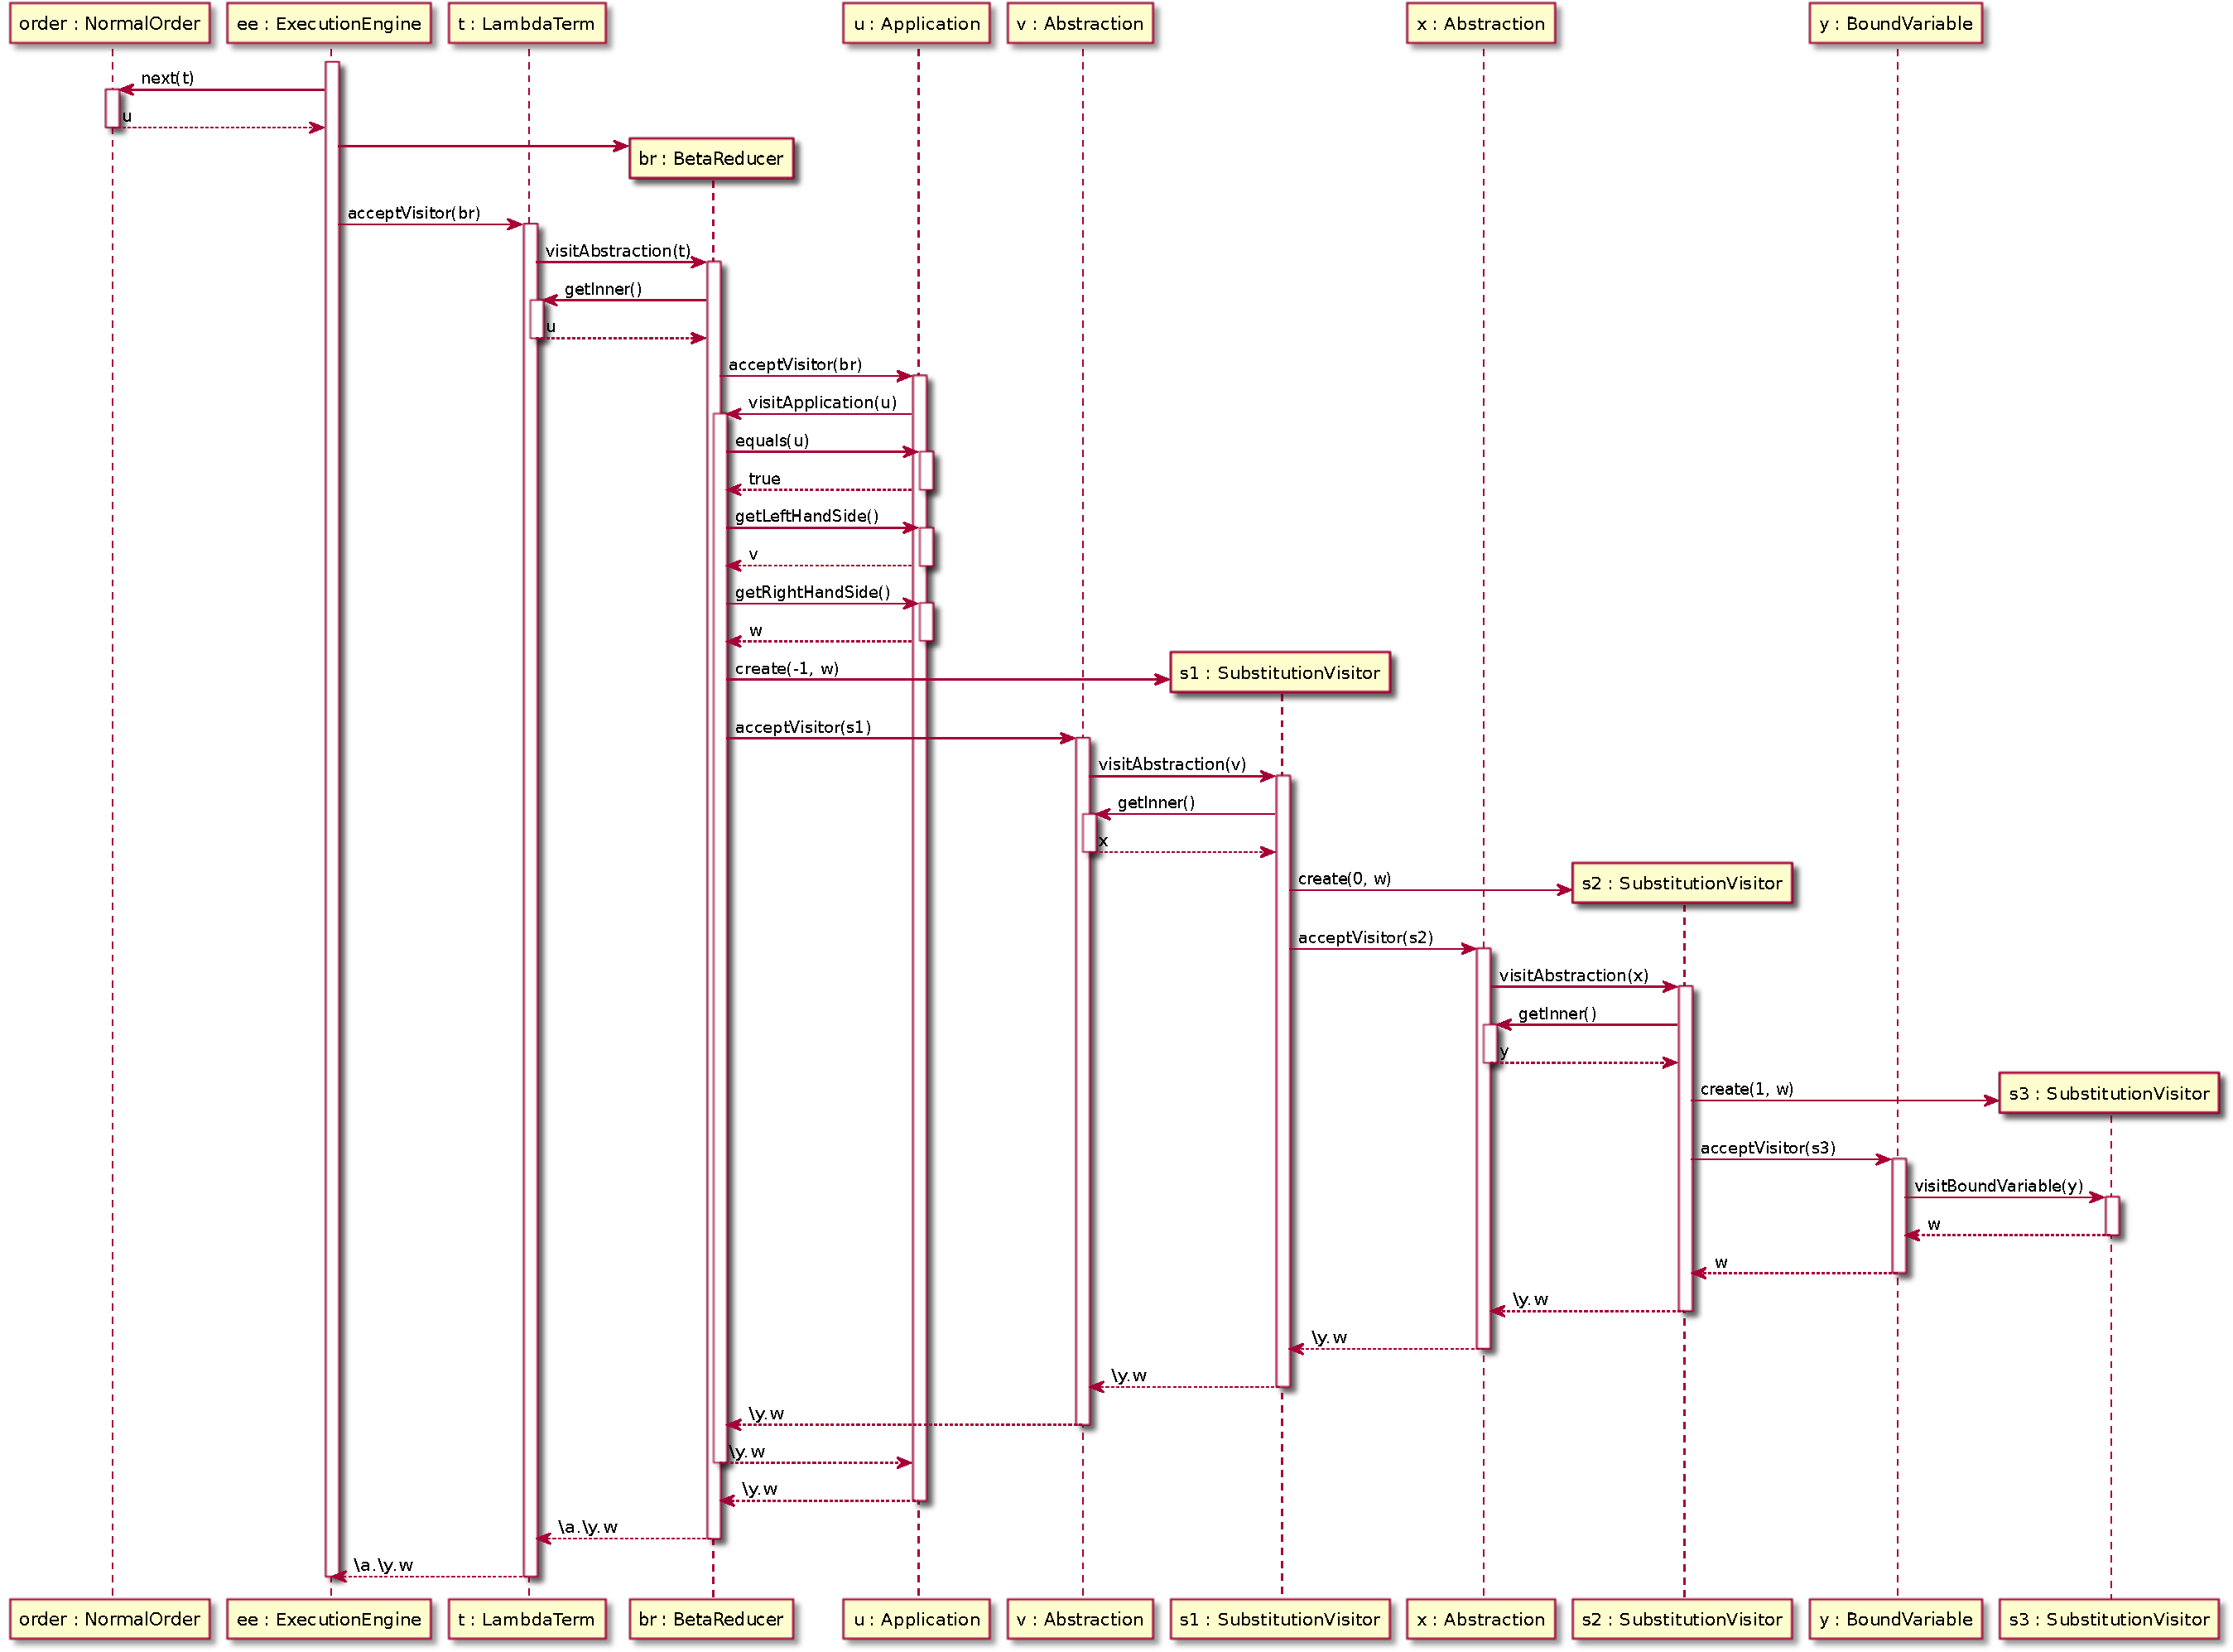
\includegraphics[width=\textwidth]{sequenceDiagrams/betaReduction}
	\caption{Sequence diagram for a $\beta$-reduction. In this example, we have $t = \lambda a.((\lambda x.\lambda y.x)(\lambda x.x))$,
		$u = (\lambda x.\lambda y.x)(\lambda x.x)$, $v = \lambda x.\lambda y.x$,
		$w = \lambda x.x$, $x = \lambda y.x$ and $y = x$. Note that in the terms called
		$x$ and $y$, the variable $x$ is actually represented as the De Bruijn index $2$
		(and not as a free variable).}
\end{figure}


\end{document}
